\documentclass{standalone}
\usepackage{tikz}
\usetikzlibrary{patterns, positioning}
\usepackage[sfdefault]{ClearSans} %% option 'sfdefault' activates Clear Sans as the default text font
\usepackage[T1]{fontenc}

\begin{document}
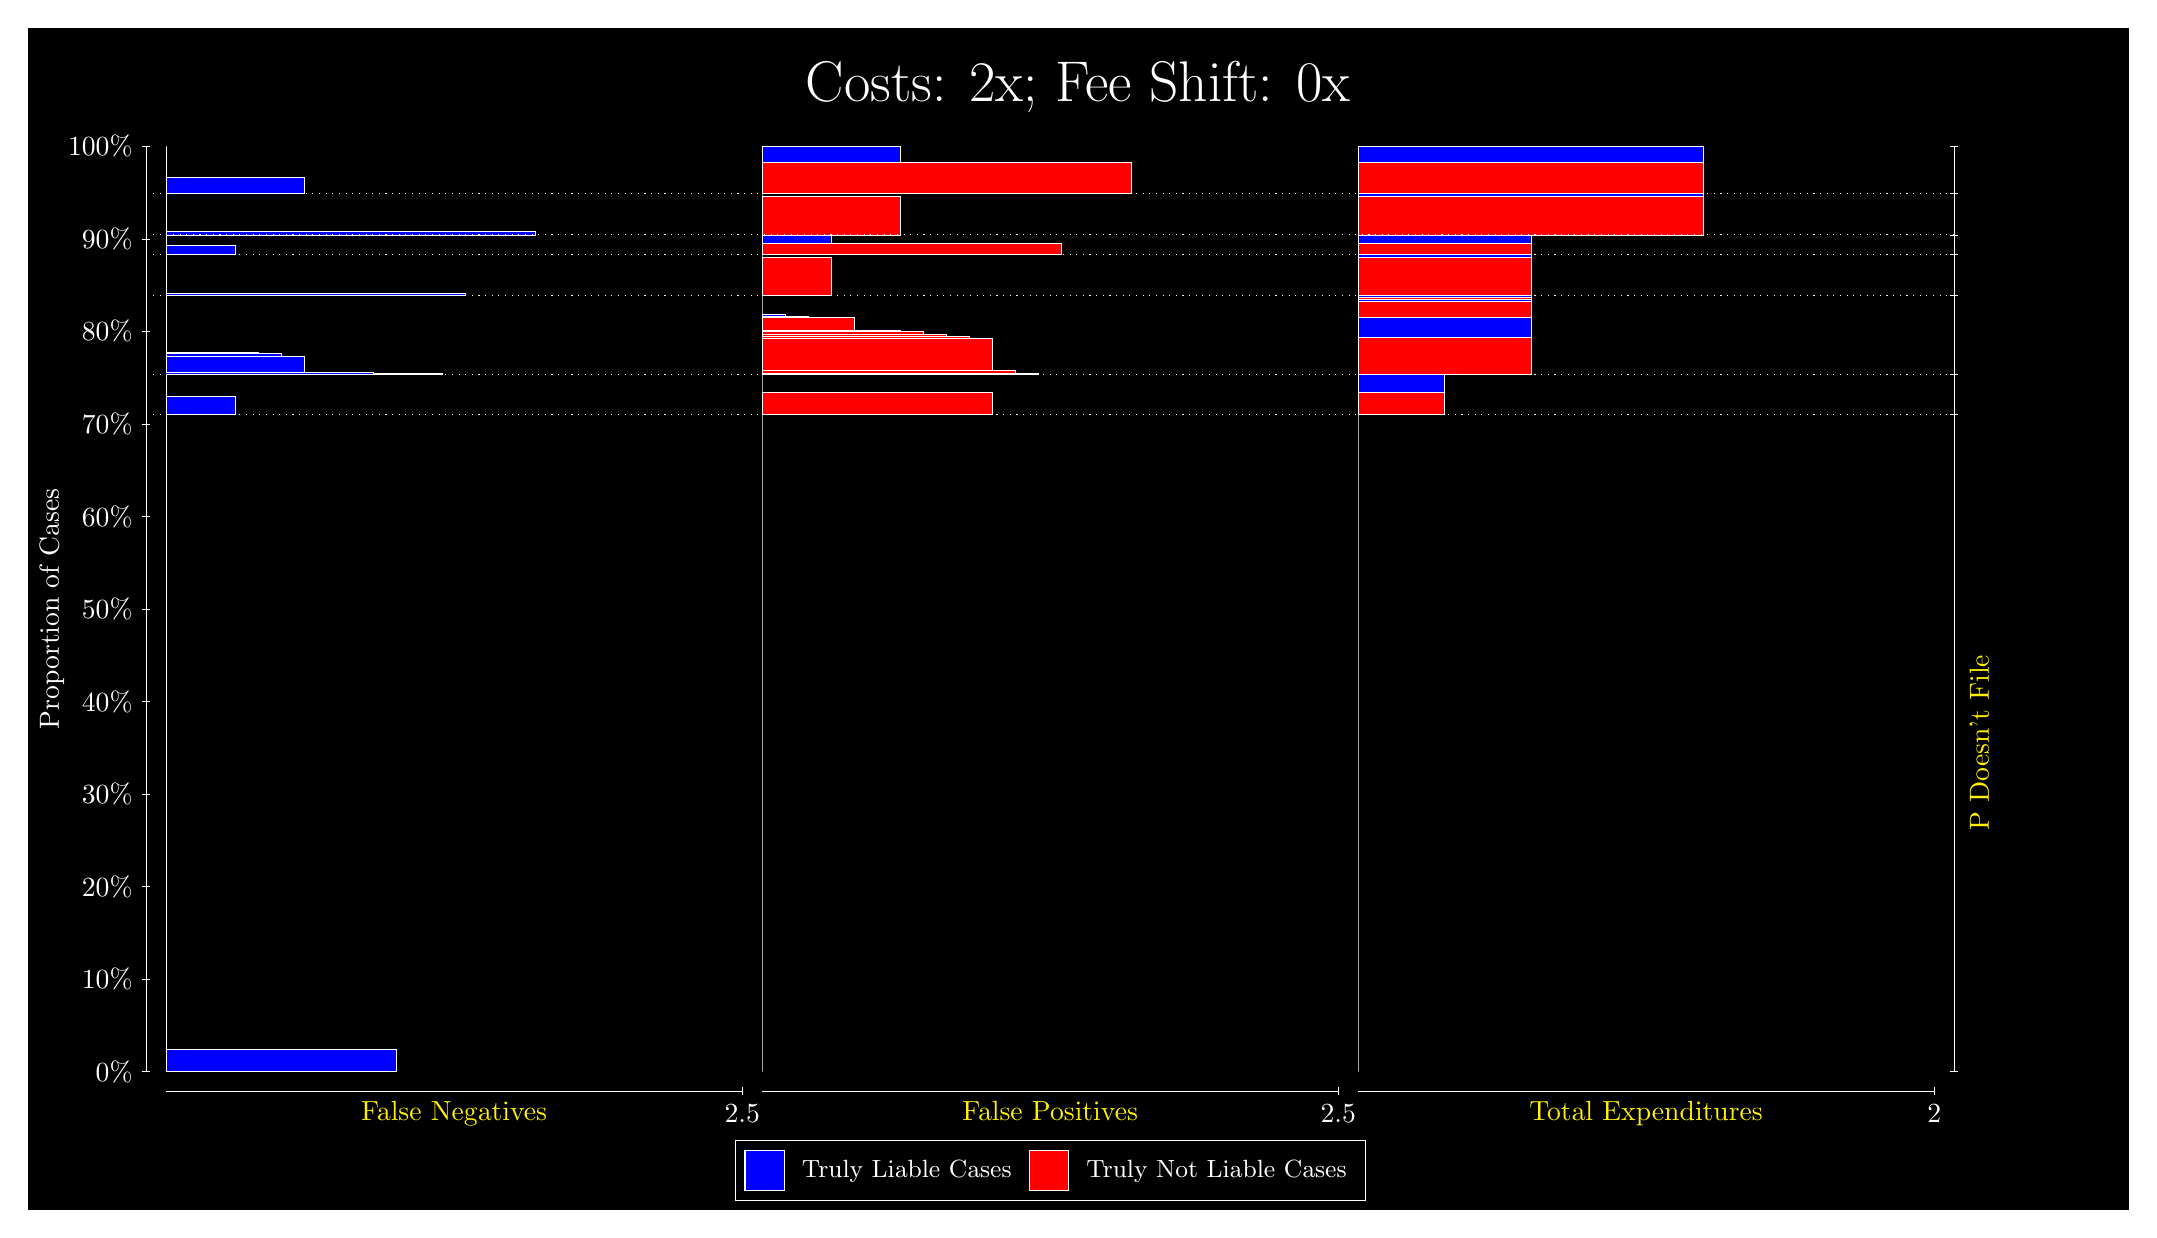
\begin{tikzpicture}
\draw[fill=black] (0,0) rectangle (26.667,15);
\draw[text=white] (0,13.5) rectangle (26.667,15) node[midway] {\huge Costs: 2x; Fee Shift: 0x};
\draw[white, very thin] (1.5,1.75) -- (1.5,13.5);
\node[rotate=90, text=white, anchor=center] at (0.3, 7.625) {Proportion of Cases};
\draw[white, very thin] (1.45,1.75) -- (1.55,1.75);
\node[text=white, anchor=east] at (1.45, 1.75) {0\%};
\draw[white, very thin] (1.45,2.925) -- (1.55,2.925);
\node[text=white, anchor=east] at (1.45, 2.925) {10\%};
\draw[white, very thin] (1.45,4.1) -- (1.55,4.1);
\node[text=white, anchor=east] at (1.45, 4.1) {20\%};
\draw[white, very thin] (1.45,5.275) -- (1.55,5.275);
\node[text=white, anchor=east] at (1.45, 5.275) {30\%};
\draw[white, very thin] (1.45,6.45) -- (1.55,6.45);
\node[text=white, anchor=east] at (1.45, 6.45) {40\%};
\draw[white, very thin] (1.45,7.625) -- (1.55,7.625);
\node[text=white, anchor=east] at (1.45, 7.625) {50\%};
\draw[white, very thin] (1.45,8.8) -- (1.55,8.8);
\node[text=white, anchor=east] at (1.45, 8.8) {60\%};
\draw[white, very thin] (1.45,9.975) -- (1.55,9.975);
\node[text=white, anchor=east] at (1.45, 9.975) {70\%};
\draw[white, very thin] (1.45,11.15) -- (1.55,11.15);
\node[text=white, anchor=east] at (1.45, 11.15) {80\%};
\draw[white, very thin] (1.45,12.325) -- (1.55,12.325);
\node[text=white, anchor=east] at (1.45, 12.325) {90\%};
\draw[white, very thin] (1.45,13.5) -- (1.55,13.5);
\node[text=white, anchor=east] at (1.45, 13.5) {100\%};

\draw[white, very thin] (24.457,1.75) -- (24.457,13.5);
\draw[white, very thin] (24.407,1.75) -- (24.507,1.75);
\node[anchor=west] at (24.407, 1.75) {};
\draw[white, very thin] (24.407,10.099) -- (24.507,10.099);
\node[anchor=west] at (24.407, 10.099) {};
\draw[white, very thin] (24.407,10.606) -- (24.507,10.606);
\node[anchor=west] at (24.407, 10.606) {};
\draw[white, very thin] (24.407,11.604) -- (24.507,11.604);
\node[anchor=west] at (24.407, 11.604) {};
\draw[white, very thin] (24.407,12.127) -- (24.507,12.127);
\node[anchor=west] at (24.407, 12.127) {};
\draw[white, very thin] (24.407,12.375) -- (24.507,12.375);
\node[anchor=west] at (24.407, 12.375) {};
\draw[white, very thin] (24.407,12.904) -- (24.507,12.904);
\node[anchor=west] at (24.407, 12.904) {};
\draw[white, very thin] (24.407,13.5) -- (24.507,13.5);
\node[anchor=west] at (24.407, 13.5) {};

\draw[white, very thin, fill=blue] (1.75,1.75) rectangle (4.6775,2.0323);
\draw[white, very thin, fill=red] (1.75,2.0323) rectangle (1.75,10.099);
\draw[white, very thin, fill=blue] (1.75,10.099) rectangle (2.6283,10.326);
\draw[white, very thin, fill=red] (1.75,10.326) rectangle (1.75,10.606);
\draw[white, very thin, fill=blue] (1.75,10.606) rectangle (5.2631,10.616);
\draw[white, very thin, fill=blue] (1.75,10.616) rectangle (4.9703,10.617);
\draw[white, very thin, fill=blue] (1.75,10.617) rectangle (4.6775,10.619);
\draw[white, very thin, fill=blue] (1.75,10.619) rectangle (4.3848,10.626);
\draw[white, very thin, fill=blue] (1.75,10.626) rectangle (4.3848,10.627);
\draw[white, very thin, fill=blue] (1.75,10.627) rectangle (4.092,10.631);
\draw[white, very thin, fill=blue] (1.75,10.631) rectangle (3.7993,10.635);
\draw[white, very thin, fill=blue] (1.75,10.635) rectangle (3.5065,10.839);
\draw[white, very thin, fill=blue] (1.75,10.839) rectangle (3.2138,10.874);
\draw[white, very thin, fill=blue] (1.75,10.874) rectangle (2.921,10.884);
\draw[white, very thin, fill=red] (1.75,10.884) rectangle (1.75,11.604);
\draw[white, very thin, fill=blue] (1.75,11.604) rectangle (5.5558,11.637);
\draw[white, very thin, fill=red] (1.75,11.637) rectangle (1.75,12.127);
\draw[white, very thin, fill=blue] (1.75,12.127) rectangle (2.6283,12.239);
\draw[white, very thin, fill=red] (1.75,12.239) rectangle (1.75,12.375);
\draw[white, very thin, fill=blue] (1.75,12.375) rectangle (6.4341,12.419);
\draw[white, very thin, fill=red] (1.75,12.419) rectangle (1.75,12.904);
\draw[white, very thin, fill=blue] (1.75,12.904) rectangle (3.5065,13.102);
\draw[white, very thin, fill=red] (1.75,13.102) rectangle (1.75,13.5);
\draw[white, very thin, fill=red] (9.3189,1.75) rectangle (9.3189,9.8167);
\draw[white, very thin, fill=blue] (9.3189,9.8167) rectangle (9.3189,10.099);
\draw[white, very thin, fill=red] (9.3189,10.099) rectangle (12.246,10.379);
\draw[white, very thin, fill=blue] (9.3189,10.379) rectangle (9.3189,10.606);
\draw[white, very thin, fill=red] (9.3189,10.606) rectangle (12.832,10.616);
\draw[white, very thin, fill=red] (9.3189,10.616) rectangle (12.539,10.657);
\draw[white, very thin, fill=red] (9.3189,10.657) rectangle (12.246,11.068);
\draw[white, very thin, fill=red] (9.3189,11.068) rectangle (11.954,11.089);
\draw[white, very thin, fill=red] (9.3189,11.089) rectangle (11.661,11.112);
\draw[white, very thin, fill=red] (9.3189,11.112) rectangle (11.368,11.155);
\draw[white, very thin, fill=red] (9.3189,11.155) rectangle (11.075,11.161);
\draw[white, very thin, fill=red] (9.3189,11.161) rectangle (10.783,11.167);
\draw[white, very thin, fill=red] (9.3189,11.167) rectangle (10.49,11.325);
\draw[white, very thin, fill=blue] (9.3189,11.325) rectangle (9.9044,11.336);
\draw[white, very thin, fill=blue] (9.3189,11.336) rectangle (9.6116,11.37);
\draw[white, very thin, fill=blue] (9.3189,11.37) rectangle (9.3189,11.604);
\draw[white, very thin, fill=red] (9.3189,11.604) rectangle (10.197,12.093);
\draw[white, very thin, fill=blue] (9.3189,12.093) rectangle (9.3189,12.127);
\draw[white, very thin, fill=red] (9.3189,12.127) rectangle (13.125,12.263);
\draw[white, very thin, fill=blue] (9.3189,12.263) rectangle (10.197,12.375);
\draw[white, very thin, fill=red] (9.3189,12.375) rectangle (11.075,12.86);
\draw[white, very thin, fill=blue] (9.3189,12.86) rectangle (9.3189,12.904);
\draw[white, very thin, fill=red] (9.3189,12.904) rectangle (14.003,13.302);
\draw[white, very thin, fill=blue] (9.3189,13.302) rectangle (11.075,13.5);
\draw[white, very thin, fill=red] (16.888,1.75) rectangle (16.888,9.8167);
\draw[white, very thin, fill=blue] (16.888,9.8167) rectangle (16.888,10.099);
\draw[white, very thin, fill=red] (16.888,10.099) rectangle (17.986,10.379);
\draw[white, very thin, fill=blue] (16.888,10.379) rectangle (17.986,10.606);
\draw[white, very thin, fill=red] (16.888,10.606) rectangle (19.083,11.081);
\draw[white, very thin, fill=blue] (16.888,11.081) rectangle (19.083,11.324);
\draw[white, very thin, fill=red] (16.888,11.324) rectangle (19.083,11.536);
\draw[white, very thin, fill=blue] (16.888,11.536) rectangle (19.083,11.556);
\draw[white, very thin, fill=red] (16.888,11.556) rectangle (19.083,11.589);
\draw[white, very thin, fill=blue] (16.888,11.589) rectangle (19.083,11.604);
\draw[white, very thin, fill=red] (16.888,11.604) rectangle (19.083,12.093);
\draw[white, very thin, fill=blue] (16.888,12.093) rectangle (19.083,12.127);
\draw[white, very thin, fill=red] (16.888,12.127) rectangle (19.083,12.263);
\draw[white, very thin, fill=blue] (16.888,12.263) rectangle (19.083,12.375);
\draw[white, very thin, fill=red] (16.888,12.375) rectangle (21.279,12.86);
\draw[white, very thin, fill=blue] (16.888,12.86) rectangle (21.279,12.904);
\draw[white, very thin, fill=red] (16.888,12.904) rectangle (21.279,13.302);
\draw[white, very thin, fill=blue] (16.888,13.302) rectangle (21.279,13.5);
\draw[white, dotted] (1.5,10.099) -- (24.457,10.099);
\draw[white, dotted] (1.5,10.606) -- (24.457,10.606);
\draw[white, dotted] (1.5,11.604) -- (24.457,11.604);
\draw[white, dotted] (1.5,12.127) -- (24.457,12.127);
\draw[white, dotted] (1.5,12.375) -- (24.457,12.375);
\draw[white, dotted] (1.5,12.904) -- (24.457,12.904);
\draw[white, very thin] (1.75,1.5) -- (9.0689,1.5);
\node[text=yellow, anchor=north] at (5.4094, 1.5) {False Negatives};
\draw[white, very thin] (9.0689,1.45) -- (9.0689,1.55);
\node[text=white, anchor=north] at (9.0689, 1.45) {2.5};

\draw[white, very thin] (9.3189,1.5) -- (16.638,1.5);
\node[text=yellow, anchor=north] at (12.978, 1.5) {False Positives};
\draw[white, very thin] (16.638,1.45) -- (16.638,1.55);
\node[text=white, anchor=north] at (16.638, 1.45) {2.5};

\draw[white, very thin] (16.888,1.5) -- (24.207,1.5);
\node[text=yellow, anchor=north] at (20.547, 1.5) {Total Expenditures};
\draw[white, very thin] (24.207,1.45) -- (24.207,1.55);
\node[text=white, anchor=north] at (24.207, 1.45) {2};

\node[text=yellow, centered, rotate=90] at (24.777, 5.9245) {P Doesn't File};







\draw (12.978300999999998,1.5) node[draw=none] (baseCoordinate) {};
\begin{scope}[align=center]
        \matrix[scale=0.5, draw=white, below=0.5cm of baseCoordinate, nodes={draw}, column sep=0.1cm]{
            \node[rectangle, draw, minimum width=0.5cm, minimum height=0.5cm, fill=blue] {}; &
            \node[draw=none, font=\small, text=white] (B) {Truly Liable Cases}; &
            \node[rectangle, draw, minimum width=0.5cm, minimum height=0.5cm, fill=red] {}; &
            \node[draw=none, font=\small, text=white] (B) {Truly Not Liable Cases}; \\
            };
\end{scope}

\end{tikzpicture}
\end{document}